%\documentclass[a4paper]{article}
%\usepackage[top=1in, bottom=1.25in, left=1.25in, right=1.25in]{geometry}
%\usepackage{amsmath}
%\usepackage{multicol}
%\usepackage{graphicx}
%\usepackage{subfig}
%\usepackage{amssymb}
%%\RequirePackage{ltxcmds}[2010/12/07]
%%opening
%\title{Linear Filtering in Frequency-Domain}
%\author{ }
%\date{ }
%\begin{document}
%
%\maketitle
%Python code highlighting
\definecolor{mygreen}{rgb}{0,0.6,0}
\definecolor{mygray}{rgb}{0.5,0.5,0.5}
\definecolor{mymauve}{rgb}{0.58,0,0.82}

\lstset{ %
	backgroundcolor=\color{white},   % choose the background color; you must add \usepackage{color} or \usepackage{xcolor}; should come as last argument
	basicstyle=\footnotesize,        % the size of the fonts that are used for the code
	breakatwhitespace=false,         % sets if automatic breaks should only happen at whitespace
	breaklines=true,                 % sets automatic line breaking
	captionpos=b,                    % sets the caption-position to bottom
	commentstyle=\color{mygreen},    % comment style
	deletekeywords={...},            % if you want to delete keywords from the given language
	escapeinside={\%*}{*)},          % if you want to add LaTeX within your code
	extendedchars=true,              % lets you use non-ASCII characters; for 8-bits encodings only, does not work with UTF-8
	frame=single,	                   % adds a frame around the code
	keepspaces=true,                 % keeps spaces in text, useful for keeping indentation of code (possibly needs columns=flexible)
	keywordstyle=\color{blue},       % keyword style
	language=Octave,                 % the language of the code
	morekeywords={*,...},            % if you want to add more keywords to the set
	numbers=left,                    % where to put the line-numbers; possible values are (none, left, right)
	numbersep=5pt,                   % how far the line-numbers are from the code
	numberstyle=\tiny\color{mygray}, % the style that is used for the line-numbers
	rulecolor=\color{black},         % if not set, the frame-color may be changed on line-breaks within not-black text (e.g. comments (green here))
	showspaces=false,                % show spaces everywhere adding particular underscores; it overrides 'showstringspaces'
	showstringspaces=false,          % underline spaces within strings only
	showtabs=false,                  % show tabs within strings adding particular underscores
	stepnumber=2,                    % the step between two line-numbers. If it's 1, each line will be numbered
	stringstyle=\color{mymauve},     % string literal style
	tabsize=2,	                   % sets default tabsize to 2 spaces
	title=\lstname                   % show the filename of files included with \lstinputlisting; also try caption instead of title
}
\clearpage
\section{Filter}
\subsection*{Test setup}
\begin{figure}[h]
	\centering
	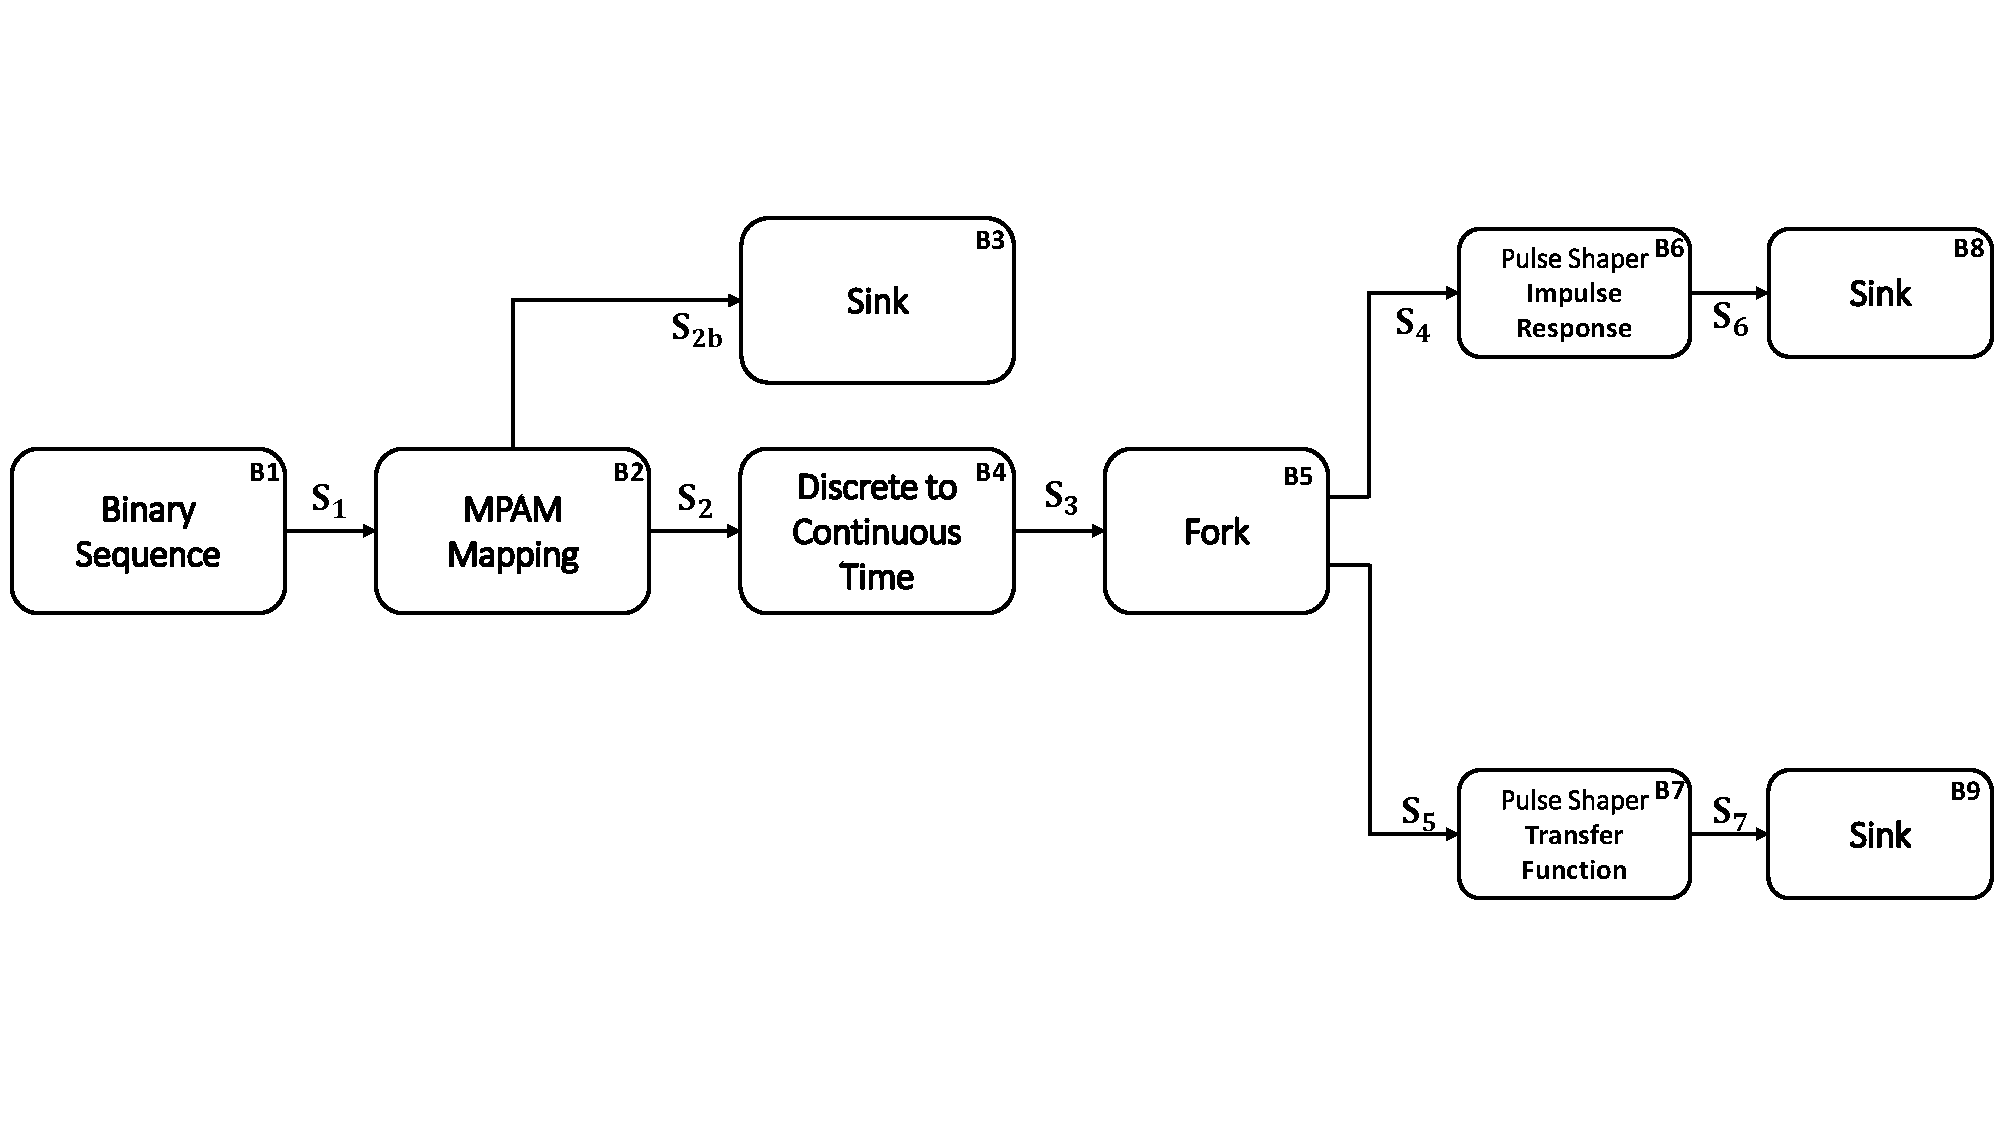
\includegraphics[width=14cm]{./algorithms/filter/figures/Test_Filter_Dia.pdf}
	\caption{Filter test setup}
	\label{FilterTest}
\end{figure}

\subsection*{Test example}
This section explains the how to use the pulse shaping filter to work in the time and frequency domain.\\
\textbf{Step 1} : Open the folder namely \textbf{filter\_test} by following the path  "/algorithms/filter/filter\_test".\\ 
\textbf{Step 2} : Find the \textbf{filter\_test.vcxproj} file in the same folder and open it.\\
In this project file, find \textit{filter\_test.cpp} in $Source Files$ section and click on it. This file is an example of using $PulseShaper$ in the time and frequency domain.\\
\lstinputlisting[language=C++, caption=filter\_test.cpp code]{../../algorithms/filter/filter_test/filter_test.cpp}
\textbf{Step 3} : Set the domain of the filter to \textit{time} or \textit{frequency} using \textbf{setFilterDomianType} and select type of the filter to \textit{ RaisedCosine, Gaussian} or \textit{Square} using \textbf{setFilterType}.\\ \\
\textbf{Step 4} : Run the code and compare the resulting signals \textbf{S6.sgn} and \textbf{S7.sgn} using visualizer.\\
The \textit{filter.h} file contains two class namely \textbf{FilterRoot} and \textbf{PulseShaperFilter}.\\
\lstinputlisting[language=C++, caption=filter.h code]{../../algorithms/filter/filter.h}
The code of the \textit{filter.cpp} contains thee definitions namely; initialize, initialize\_FilterRoot and runBlock.
\lstinputlisting[language=C++, caption=filter.cpp code]{../../algorithms/filter/filter.cpp}
\newpage
\subsection*{Results}
The following two graphs displays the result of \textbf{S6.sgn} and \textbf{S7.sgn}.
\begin{figure}[h]
	\centering
	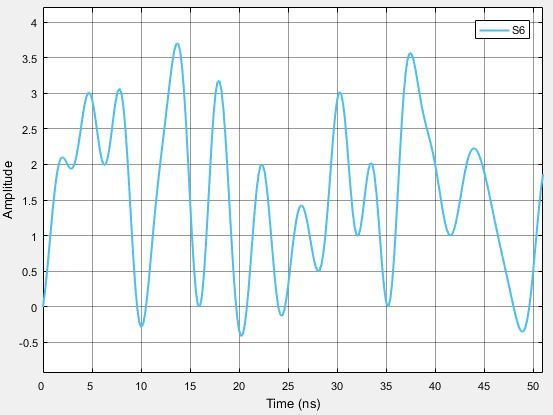
\includegraphics[width=10cm]{./algorithms/filter/figures/S6.jpg}
	\caption{S6.sgn signal}
	\label{S6}
\end{figure}
\begin{figure}[h]
	\centering
	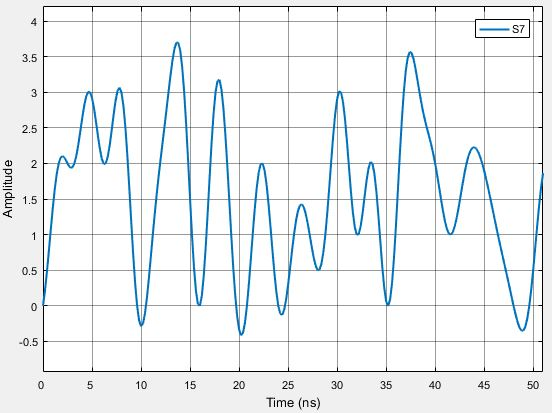
\includegraphics[width=10cm]{./algorithms/filter/figures/S7.jpg}
	\caption{S7.sgn signal}
	\label{S7}
\end{figure}

\subsection*{Remarks}

\newpage
%%%%%%%%%%%%%%%%%%%%%%%%%%%%%%%%%%%%%%%%%%%%%%%%%%%%%%%%%%%%%%%%%%%%%%%%%%%%%%%%%%%%%%%%%%%%%%%%%%%%%%%%%%%%
% References
%%%%%%%%%%%%%%%%%%%%%%%%%%%%%%%%%%%%%%%%%%%%%%%%%%%%%%%%%%%%%%%%%%%%%%%%%%%%%%%%%%%%%%%%%%%%%%%%%%%%%%%%%%%%

\renewcommand{\bibname}{References}
%
%\bibliographystyle{myIEEEtran}
%\bibliography{./algorithms/fft/fft}
%
%

\cleardoublepage


%%%%%%%%%%%%%%%%%%%%%%%%%%%%%%%%%%%%%%%%%%%%%%%%%%%%%
%%%%%%%%%%% Example flowchart START %%%%%%%%%%%%%%%%%
%\tikzstyle{decision} = [diamond, draw, fill=blue!20,
%text width=4.5em, text badly centered, node distance=3cm, inner sep=0pt]
%\tikzstyle{block} = [rectangle, draw, fill=blue!20,
%text width=5em, text centered, rounded corners, minimum height=4em]
%\tikzstyle{line} = [draw, -latex']
%\tikzstyle{cloud} = [draw, ellipse,fill=red!20, node distance=3cm,
%minimum height=2em]
%\begin{tikzpicture}[node distance = 2cm, auto]
%% Place nodes
%\node [block] (init) {initialize model};
%\node [cloud, left of=init] (expert) {expert};
%\node [cloud, right of=init] (system) {system};
%\node [block, below of=init] (identify) {identify candidate models};
%\node [block, below of=identify] (evaluate) {evaluate candidate models};
%\node [block, left of=evaluate, node distance=3cm] (update) {update model};
%\node [decision, below of=evaluate] (decide) {is best candidate better?};
%\node [block, below of=decide, node distance=3cm] (stop) {stop};
%% Draw edges
%%\path [line] (init) -- (identify);
%\path [line] (identify) -- (evaluate);
%\path [line] (evaluate) -- (decide);
%\path [line] (decide) -| node [near start] {yes} (update);
%\path [line] (update) |- (identify);
%\path [line] (decide) -- node {no}(stop);
%\path [line,dashed] (expert) -- (init);
%\path [line,dashed] (system) -- (init);
%\path [line,dashed] (system) |- (evaluate);
%\end{tikzpicture}
%%%%%%%%%%% Example flowchart END %%%%%%%%%%%%%%%%%
%%%%%%%%%%%%%%%%%%%%%%%%%%%%%%%%%%%%%%%%%%%%%%%%%%%


%\end{document}

